\section{Auswertung}
\label{sec:Auswertung}


\subsection{Zählrohr-Charakteristik}

Im Folgenden wird die Zählrohr-Charakteristik eines Halogenzählrohrs bestimmt. Die Werte für die angelegte Spannung $U$ und die Anzahl der gemessenen Impulse sind in Tab. \ref{taba} dargestellt. 

\begin{table}\caption{Die Länge der Zylinder und die Spannung mit den jeweiligen Zeitenpunkten der Ausschläge.}
\label{taba}
\centering
\sisetup{round-mode = places, round-precision=2, round-integer-to-decimal=true}
\begin{tabular}{S[]S[]S[]S[]S[]} 
\toprule
{$l/ \si{\milli\meter}$} & {$U_1/ \si{\volt}$} & {$t_1/ \si{\micro\second}$} & {$U_2/ \si{\volt}$} & {$t_2/ \si{\micro\second}$}\\
\midrule
120.8 & 1.29 & 0.6 & 0.17 & 88.7\\
102.3 & 1.27 & 0.5 & 0.2 & 76.5\\
80.5 & 1.33 & 0.6 & 0.76 & 59.8\\
40.4 & 1.33 & 0.5 & 1.34 & 30.2\\
31.1 & 1.29 & 0.5 & 1.37 & 23.8\\
\bottomrule
\end{tabular}\end{table}

\noindent Die Anzahl der Impulse wird in einer Zeit von 
\begin{equation*}
    \Delta t = \SI{130}{\second}
\end{equation*}
gemessen. 
Die normierten und fehlerbehafteten Werte für die Anzahl der Impulse befinden sich in Tab. \ref{tab1}. 

\begin{table}\caption{Der maximale Drehimpuls $L$, der Gesamtspin $S$ und der Gesamtdrehimpuls $J$ ergeben sich zum Landé-Faktor $g_\text{J}$ für die vier verschiedenen Elemente.}
\label{tab1}
\centering
\sisetup{round-mode = places, round-precision=2, round-integer-to-decimal=true}
\begin{tabular}{S[]S[]S[]S[]} 
\toprule
{$L$} & {$S$} & {$J$} & {$g_\text{J}$}\\
\midrule
5.0 & 1.0 & 4.0 & 0.8\\
0.0 & 3.5 & 3.5 & 2.0\\
6.0 & 1.5 & 4.5 & 0.7272727272727273\\
5.0 & 2.5 & 7.5 & 1.3333333333333333\\
\bottomrule
\end{tabular}\end{table}

\noindent In Abb. \ref{fig1} sind diese Werte gegeneinander aufgetragen und es wird eine Ausgleichsgerade im Bereich von $\num{360}$ bis $\SI{620}{\volt}$ mit der allgemeinen Gleichung \eqref{linReg} für die lineare Regressionen bestimmt. 

\begin{figure}
    \centering
    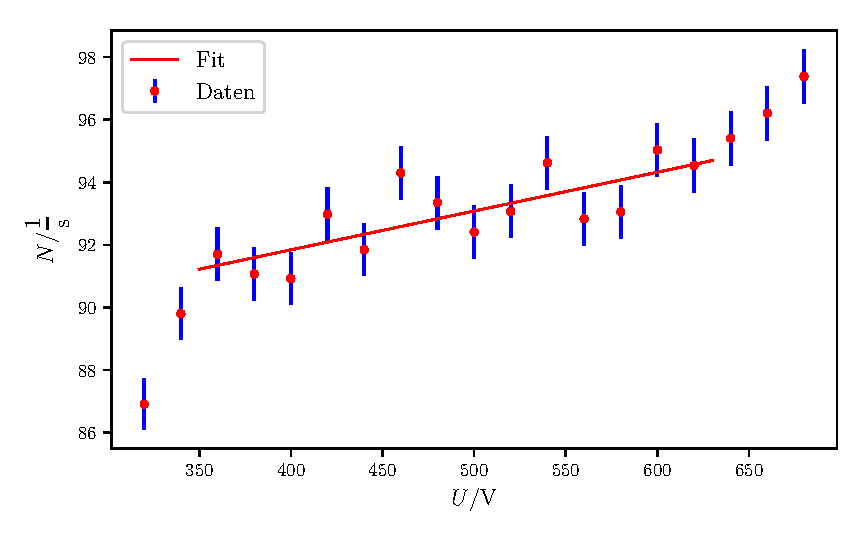
\includegraphics[width=15cm, height=9cm]{build/plot1.pdf}
    \caption{Die Zählrate $N$ ist gegen die angelegte Spannung $U$ aufgetragen. Es sind die Daten mit Fehlern sowie eine Ausgleichsgerade im Bereich von $\num{360}$ bis $\SI{620}{\volt}$ eingetragen.}
    \label{fig1}
\end{figure}

\noindent Die lineare Regression ergibt als Parameter

\begin{align*} 
   m &= \SI{0.012}{\per\volt\per\second} \\
   n &= \SI{86.88}{\per\second}.
\end{align*}

\noindent Mit diesen Parametern lässt sich aus den Werten für die Anzahl bei \num{450} und \SI{550}{\volt} die Steigung des Plateaus mit Gleichung \eqref{steigung} bestimmen.
Die Steigung des Plateaus beträgt 

\begin{align*} 
    m_\text{Plateau} = \num{1.33} \frac{\si{\percent}}{\SI{100}{\volt}}.
\end{align*}

\subsection{Totzeitbestimmung}

Bei einer Spannung von $\SI{500}{\volt}$ ergibt sich durch das Ablesen vom Oszilloskop (Abb. \ref{foto}) eine Totzeit von 
\begin{equation*}
    T_\text{Tot,1} = \SI{54(10)}{\micro\second}.
\end{equation*}

\begin{figure}
    \centering
    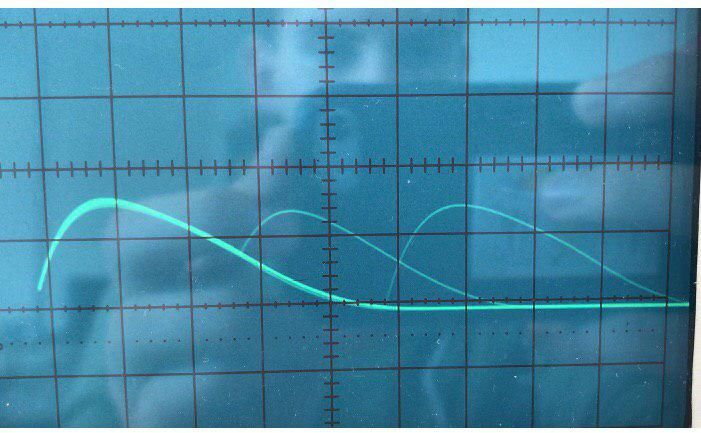
\includegraphics[width=12cm, height=8cm]{build/foto.jpg}
    \caption{Das Foto des Bildschrims des Oszilloskops. Die $x$-Achse entspricht der Zeit (\SI{20}{\micro\second} pro Kästchen) und die $y$-Achse (\SI{1}{\volt} pro Kästchen) der Spannung. Die beiden rechten Kurven entsprechen den Nachentladungen.}
    \label{foto}
\end{figure}

\noindent Die Totzeit lässt sich auch durch die Zwei-Quellen-Methode berechnen. 
Bei der Messung haben sich für die erste und zweite Quelle, sowie für die Kombination aus beiden folgende Werte ergeben
\begin{align*} 
   N_1 &= 9730 \frac{1}{\SI{60}{\second}}\\
   N_2 &= 11918 \frac{1}{\SI{60}{\second}} \\
   N_{1+2} &= 21187 \frac{1}{\SI{60}{\second}}.
\end{align*}

\noindent Diese Werte werden durch die Messdauer von
\begin{equation*}
    \Delta t = \SI{60}{\second}
\end{equation*}
geteilt und ein Fehler entsteht ebenfalls dadurch %?

\begin{align*} 
   N_1 &= \num{162.17(10)} \si{\per\second}\\
   N_2 &= \num{198.63(11)} \si{\per\second} \\
   N_{1+2} &=\num{353.12(14)} \si{\per\second}.
\end{align*}

\noindent Daraus ergibt sich für die Totzeit mit Gleichung \eqref{totzeit}
ein Wert von 
\begin{equation*} 
    T_\text{Tot,2} = \SI{119.3(31)}{\micro\second}.
\end{equation*} 

\subsection{Transportierte Ladungsmenge}
In Tab. \ref{tabb} stehen die Anzahl der gemessenen Impulse und die Stromstärke bei verschiedenen angelegten Spannungen.
In Abb. \ref{fig2} sind die Spannung und die Stromstärke gegeneinander aufgetragen. 

\begin{table}\caption{Die angelegte Spannung des elektrischen Feldes innerhalb des Geiger-Müller-Zählrohrs, die Anzahl der jeweils gemessenen Impulse und der Strom innerhalb des Geiger-Müller-Zählrohrs.}
\label{tabb}
\centering
\sisetup{round-mode = places, round-precision=2, round-integer-to-decimal=true}
\begin{tabular}{c c S[]} 
\toprule
{$U / \si{\volt}$} & {$\frac{N}{\SI{130}{\second}}$} & {$I / \si{\ampere}$}\\
\midrule
320 & 11298 & 0.1\\
400 & 11820 & 0.2\\
480 & 12135 & 0.3\\
540 & 12301 & 0.35\\
560 & 12068 & 0.4\\
600 & 12354 & 0.45\\
640 & 12403 & 0.5\\
660 & 12507 & 0.55\\
680 & 12659 & 0.6\\
\bottomrule
\end{tabular}\end{table}

\begin{figure}
    \centering
    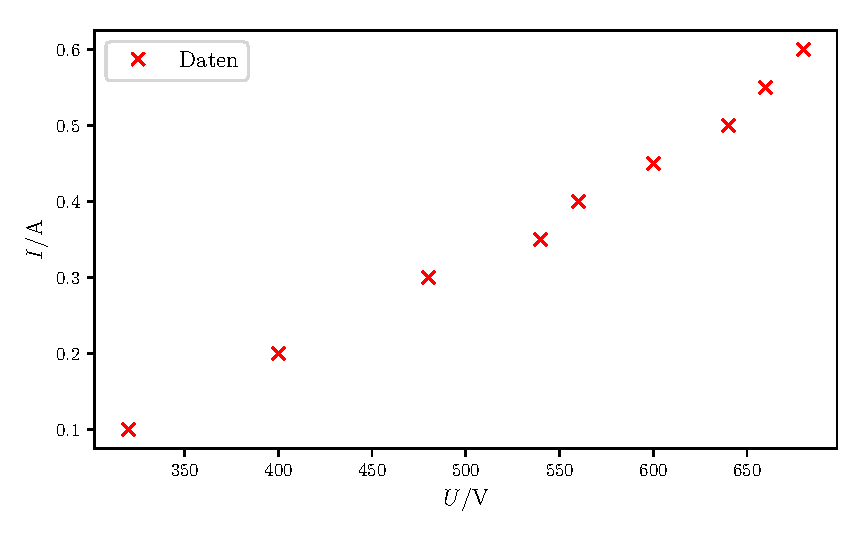
\includegraphics[width=15cm, height=9cm]{build/plot2.pdf}
    \caption{Die Stromstärke ist gegen die angelegte Spannung aufgetragen. Es sind nur die Daten eingetragen.}
    \label{fig2}
\end{figure}

\noindent Aus den Werten für die Stromstärke und der Anzahl der Impulse ergibt sich mit Gleichung \eqref{ladung} die transportierte Ladungsmenge $\Delta Q$ und daraus wiederum die transportierte Ladungsmenge in Abhängigkeit von der Elementarladung $e$. Die Ergebnisse sind in Tab. \ref{tab2} eingetragen. 
%Muss N hier nicht die Anzahl der Impulse in 130s sein?

\begin{table}\caption{Das Verhältnis des magnetischen Feldes durch die Beschleunigungsspannung aufgetragen gegen die Höhe.}
\label{tab2}
\centering
\sisetup{round-mode = places, round-precision=2, round-integer-to-decimal=true}
\begin{tabular}{S[]S[]S[]} 
\toprule
{$B_1 / \si{\henry}$} & {$B_2 / \si{\henry}$} & {$\frac{D}{(L^2 + D^2)} / \si{\per\meter}$}\\
\midrule
0.0 & 0.0 & 0.0\\
3.5649278338607584e-07 & 3.862005153349155e-07 & 0.29289724188430566\\
8.912319584651897e-07 & 8.912319584651897e-07 & 0.5827222842713544\\
1.4259711335443034e-06 & 1.396263401595464e-06 & 0.8665094112549946\\
1.9250610302848096e-06 & 1.8418793808280586e-06 & 1.1414982164090373\\
2.3885016486867084e-06 & 2.3172030920094934e-06 & 1.4052180429996723\\
2.923240823765822e-06 & 2.822234535139767e-06 & 1.6555530006898145\\
3.4223307205063282e-06 & 3.3272659782700412e-06 & 1.8907846756403912\\
\bottomrule
\end{tabular}\end{table}


